
\section{Inter-calibration {\color{blue} Nico}}
\label{se:intercalibration}

{\color{blue} More details on the intercalibration as described in Sect.~\ref{se:fp_reconstruction}} \\

{\color{blue} NB: Main beam flat field = calib $\_$ fwhm $\_$ fix}


\section{Flat field stability {\color{blue} Laurence} }
\label{se:flatfields}

The dispersion of the detector responsivity across the field of view has been characterized by estimating flat fields using the nominally focused \emph{beammap} scans described in Sect.~\ref{se:fp_reconstruction}. We have considered different kinds of flat field:
\begin{itemize}
\item Main beam flat field: the flat field for the main beam, which is the far field of the telescope estimated for the sources, is determined using the relative calibration factors obtained for the calibration in FWHM$_{0}$ beam discussed in Sect.~\ref{se:cal_HA}. These are defined as
  \begin{equation}
    G_k = \frac{S_{th}(\nu_0)\, e^{-\tau/sin(\delta)}}{A_k}, 
  \end{equation}
  where $S_{th}(\nu_0)$ is the expected flux of the source integrated in the NIKA2 bandpasses and derived at the reference frequency $\nu_0$, $\tau/sin(\delta)$ is the line-of-sight opacity measured using the \emph{skydip} method described in Sect.~\ref{se:opacities} and $A_k$ is the amplitude of a Gaussian of fixed FWHM fitted from the detector $k$ map (as $A_{c}$ in Eq.~\ref{eq:calib_fix_fwhm}).
\item Forward beam flat field: the flat field for forward beam, which is the near field of the telescope determined for the sky noise, is estimated using the correlation factor of each detector to a median common mode estimated off-source.
\end{itemize}

Figures \ref{fig:avg_mbff} and \ref{fig:avg_fbff} show the average main beam and forward beam flat fields for the three arrays. These have been constructed by combining the normalised flat fields of five \emph{beammap} scans, which were selected by thresholding the line-of-sight opacity measured in the 1-mm band, such as $\tau/sin(\delta) \leq 0.85$. The distribution for the average flat fields are shown in the bottom panel of Fig.~\ref{fig:avg_mbff} $\&$ \ref{fig:avg_fbff}.

We observe a sizable variation of the flat fields for Array 1 from the left-most side to the right-most side of the FOV: this reveals a significant change of Array 1 detector responsivities depending on their position in the FOV. Namely, this effect, the origin of which is under investigation, mainly impacts the left-most third of the array, which is referred to as the "shadow-zone''. This variation of the flat field tanslates into a broadening of the distribution. However, we verified that A1 flat field dispersions are in line with the ones of Array 3 after the detectors within the shadow-zone were flagged out using a crescent-shaped mask. The masked flat field distributions are shown in green in Fig.~\ref{fig:avg_mbff} $\&$ \ref{fig:avg_fbff}, whereas shadow-zone distributions are in red. In addition to the average flat fields, we further characterize the flat fields for individual \emph{beammap} scans. Fig.~\ref{fig:stddev_ff} shows the dispersion of the flat fields for nine \emph{beammap} scans using either the whole FOV or masking the shadow-zone. The dispersion estimates for this two cases are gathered in Table~\ref{tab:flatfields}.      

\begin{table}[h]
\begin{center}
\begin{tabular}{|l|l|c|c|c|}
\hline
 Dispersion ($\%$)    & KID selection  &  A1 & A3  & A2 \\
\hline
Main beam flat field  & all the FOV           & $34.4 \pm 3.4$    & $15.5 \pm 1.4$  &  $13.2 \pm 1.7$  \\
                      & shadow-zone excluded  & $17.0 \pm 1.1$    & $14.2 \pm 1.2$  &  $12.8 \pm 1.3$\\
\hline
Forward beam flat field  & all the FOV           & $21.6 \pm 1.4$  & $10.1 \pm 1.7$  & $5.2 \pm 0.9$   \\
                         & shadow zone excluded  & $12.2 \pm 1.6$  & $10.1 \pm 2.1$  & $4.9 \pm 1.2$ \\
\hline
\end{tabular}
\caption[Flat field dispersions]{Average flat field dispersions in percent for nine \emph{beammap} scans over all the FOV and after masking out the shadow-zone}
\end{center}
\label{tab:flatfields}
\end{table}


\begin{figure}[ht] 
\begin{center}
  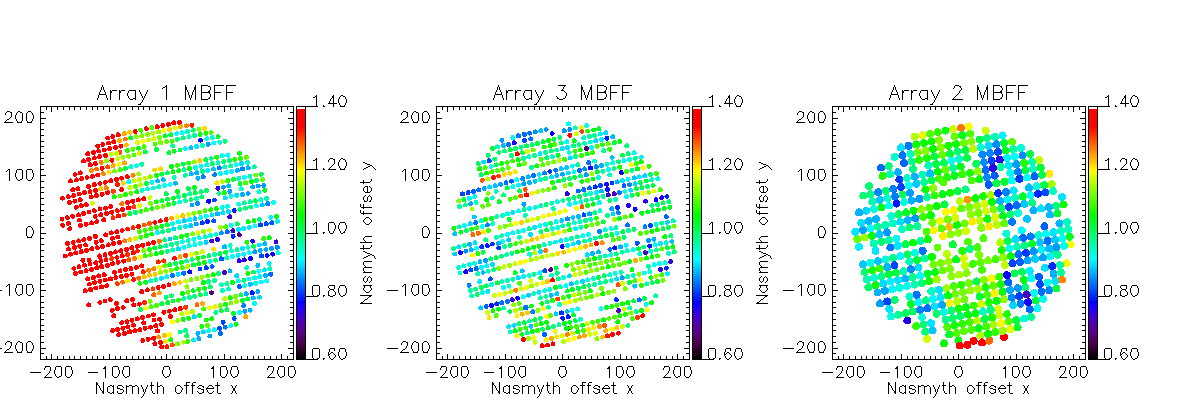
\includegraphics[width=0.95\textwidth]{Figures/FlatFields/Average_main_beam_flat_field_N2R9_10.png}
  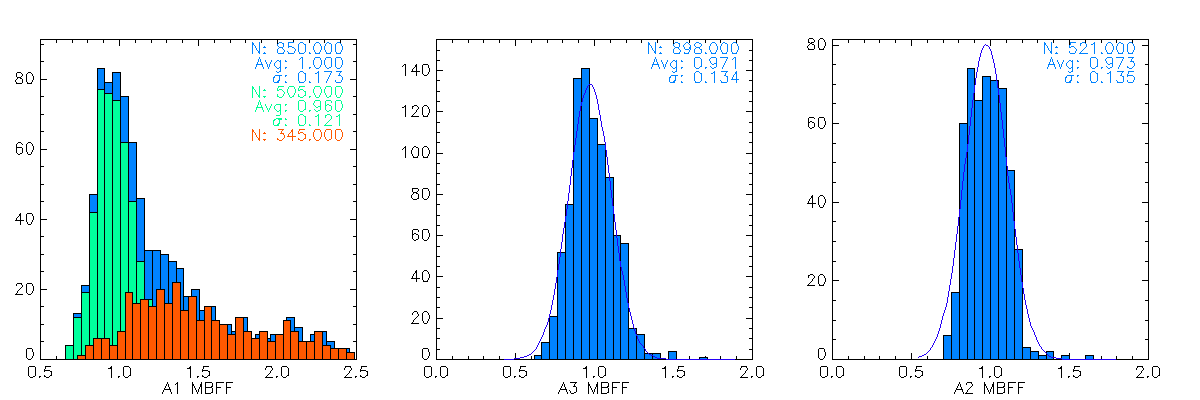
\includegraphics[width=0.8\textwidth]{Figures/FlatFields/Histo_average_main_beam_flat_field_N2R9_10.png}
\caption{Average main beam flat field for array 1, 3 and 2}
 \label{fig:avg_mbff}
\end{center}
\end{figure}

\begin{figure}[ht] 
\begin{center}
  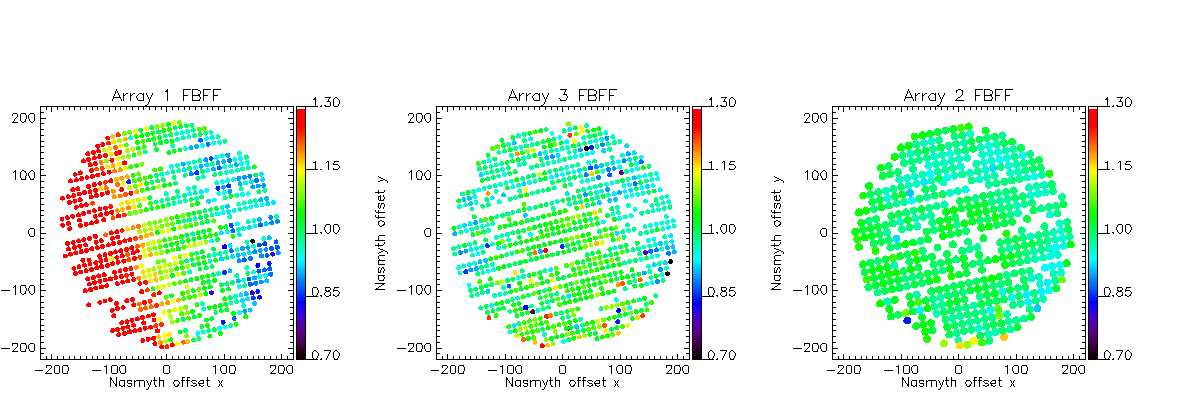
\includegraphics[width=0.95\textwidth]{Figures/FlatFields/Average_near_beam_flat_field_N2R9_10.png}
  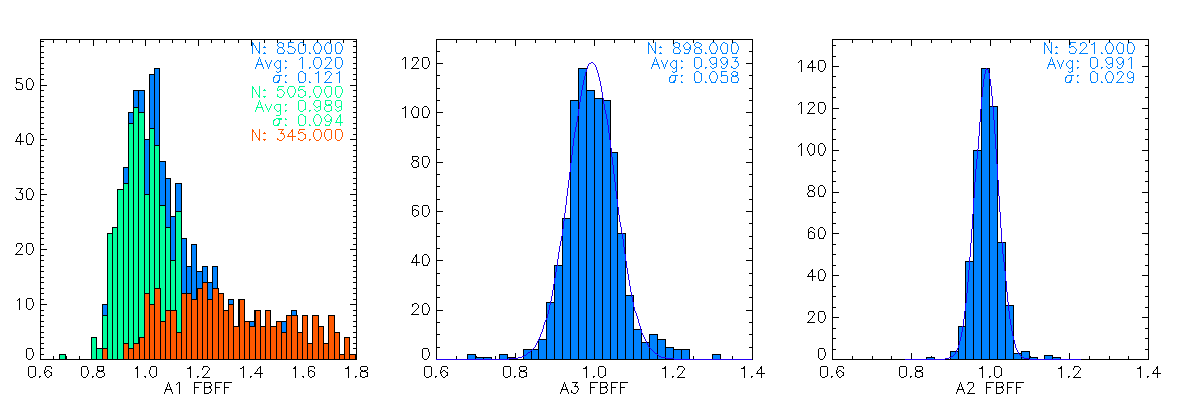
\includegraphics[width=0.8\textwidth]{Figures/FlatFields/Histo_average_near_beam_flat_field_N2R9_10.png}
\caption{Average forward efficiency flat field for array 1, 3 and 2}
 \label{fig:avg_fbff}
\end{center}
\end{figure}

\begin{figure}[ht] 
\begin{center}
  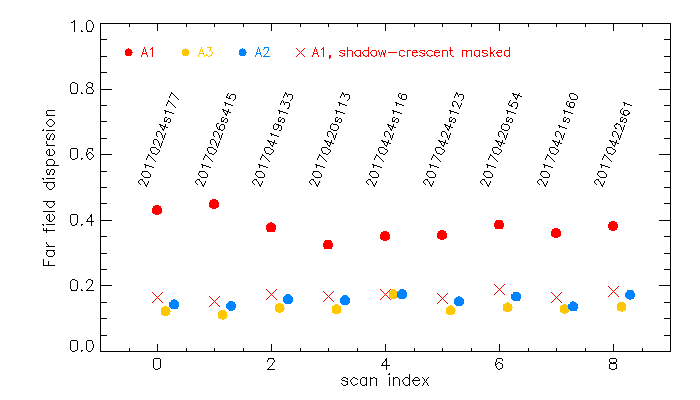
\includegraphics[width=0.6\textwidth]{Figures/FlatFields/Dispersion_main_beam_flat_field_N2R9_10_.png}
  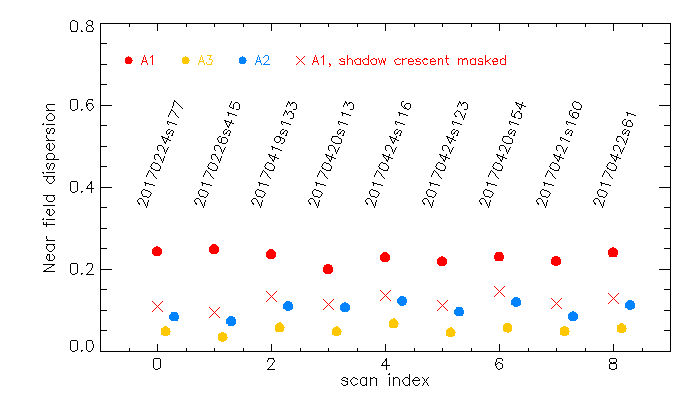
\includegraphics[width=0.6\textwidth]{Figures/FlatFields/Dispersion_forward_beam_flat_field_N2R9_10_.png}
\caption[Dispersion of the flat field for nine \emph{beammap} scans.]{The RMS dispersion of the main beam flat field (upper panel) and forward beam flat field (lower panel) are shown using all valid KIDs of Array 1 (red circles), Array 3 (orange circles) and Array 2 (blue circles), and using the KIDs located outside the Array 1 "shadow area'', which was discarded using a left crescent-shaped mask (red crosses).}
 \label{fig:stddev_ff}
\end{center}
\end{figure}
